\documentclass{article}
\usepackage[english]{babel}
\usepackage[letterpaper,top=2cm,bottom=2cm,left=3cm,right=3cm,marginparwidth=1.75cm]{geometry}
\usepackage{amsmath}
\usepackage{graphicx}
\usepackage[colorlinks=true, allcolors=blue]{hyperref}
\usepackage[numbers]{natbib}
\usepackage{listings}

\title{NOvA Production 6 Validation Task Force Contribution Summary}
\author{Larry Zhao}

\begin{document}
\maketitle

\section{Muon Neutrino Energy Estimator Validation}
Validation of the muon neutrino energy estimators compares the performance of the Spline, Regression CNN, and Transformer methods. We evaluate multiple benchmarks, including energy spectra, quantile energy spectra, bias, and resolution for each of total neutrino energy, muon energy, and hadronic energy. In addition, comparison studies of model inference performance on data and Monte-Carlo samples are completed.

\paragraph{Energy Spectra, Bias, Resolution Validation}
The energy spectra, biases, and resolutions for all three energy estimators are reasonable. The machine learning models (RegCNN, Transformer) generally outperform the Spline fit. The ML models have smaller resolutions and biases, in addition to added calibration robustness. The machine learning methods generally succeed in predicting the hadronic energy double peak truth structure, while the Spline is not capable of recreating this feature. Only the RegCNN is able to reproduce this hadronic energy double peak structure for the FHC FD sample.

\paragraph{Data/MC Validation}
In Data/MC studies, all three energy estimators display a downward shift in neutrino energy spectra for data compared to MC. The shapes of the hadronic and muon energy data also face discrepancies, particularly in the muon distribution. Further studies using updated selection cuts and cross section model tunes may improve results.

\paragraph{Calibration Shift Validation}
Previous work artificially shifted model input variables to conduct studies before the availability of official calibration shifted samples from production. The validations confirmed that the machine learning models were significantly more robust to calibration systematics than the Spline method.

\paragraph{Future Validation Work}
Current priorities are to expand the scope of validations by including resolution and bias studies in each quantile, and further evaluating changes between Prod5 and Prod6 Spline tunes. Planned future validation studies include evaluating official calibration shift samples to expand on previous validation work using self-generated calibration shift samples. Further validation studies depend on cut selections and cross section tuning, particularly to understand the Data/MC discrepancy present. Validation studies include many plots, so please refer to presentation slides referenced in the bibliography below for validation results across all detectors, horn orientations, and particle types.

% Figure~\ref{fig:lzhao-image-example} shows an example of how to include an image from the \texttt{images-lzhao} directory.

\begin{figure}[htbp]
    \centering
    \IfFileExists{images-lzhao/Numu_Energy.png}{%
        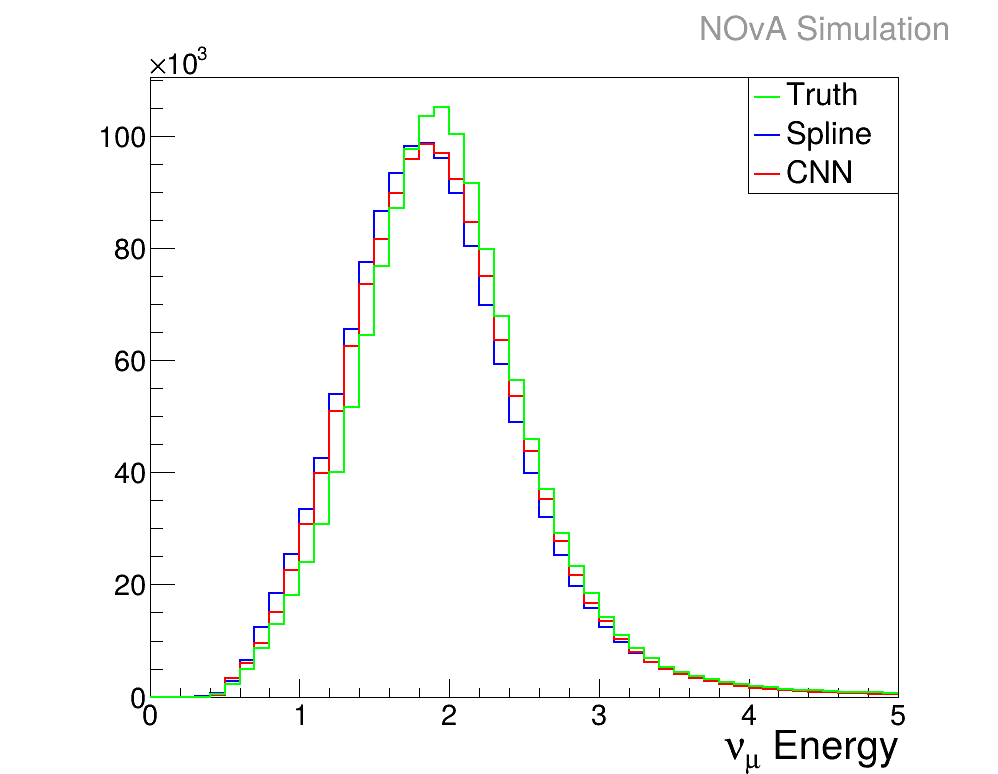
\includegraphics[width=0.7\textwidth]{images-lzhao/Numu_Energy.png}%
    }{%
        \fbox{\parbox[c][0.25\textheight][c]{0.7\textwidth}{\centering Neutrino Energy Spectrum}}%
    }
    \caption{FHC ND Neutrino Energy Spectrum.}
    \label{fig:lzhao-numu-energy-spectrum}
\end{figure}

\begin{figure}[htbp]
    \centering
    \IfFileExists{images-lzhao/Numu_Energy_Resolution_Means.png}{%
        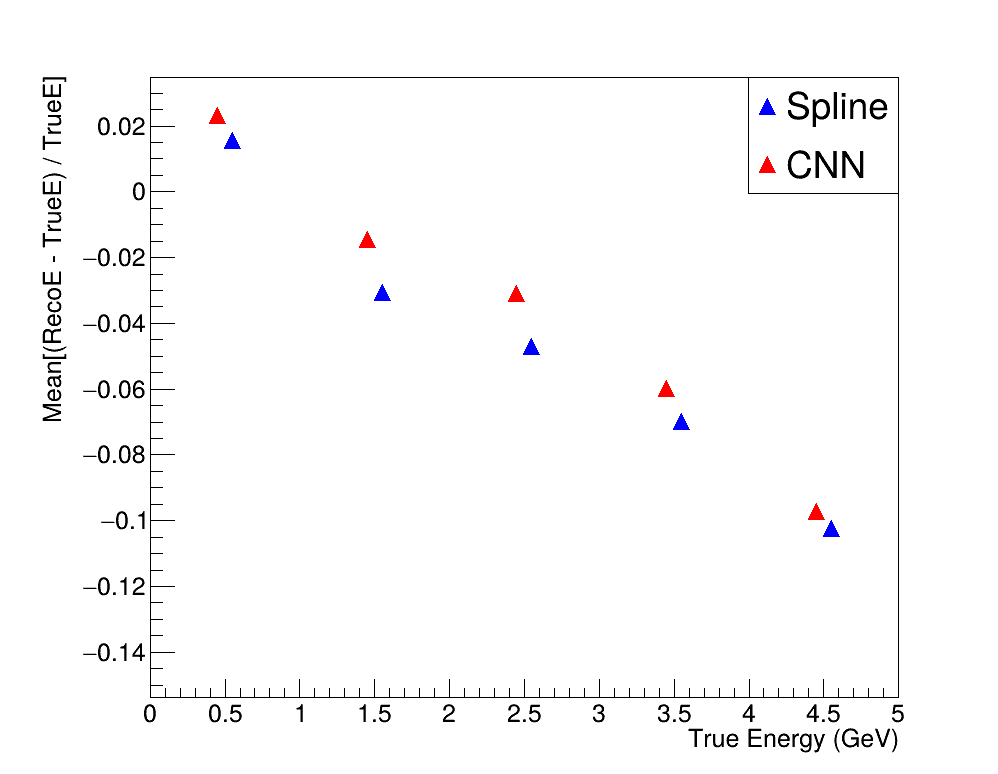
\includegraphics[width=0.7\textwidth]{images-lzhao/Numu_Energy_Resolution_Means.png}%
    }{%
        \fbox{\parbox[c][0.25\textheight][c]{0.7\textwidth}{\centering Neutrino Energy Resolution Means}}%
    }
    \caption{FHC ND Neutrino Energy Bias.}
    \label{fig:lzhao-numu-energy-bias}
\end{figure}

\begin{figure}[htbp]
    \centering
    \IfFileExists{images-lzhao/Numu_Energy_Resolution_RMSs.png}{%
        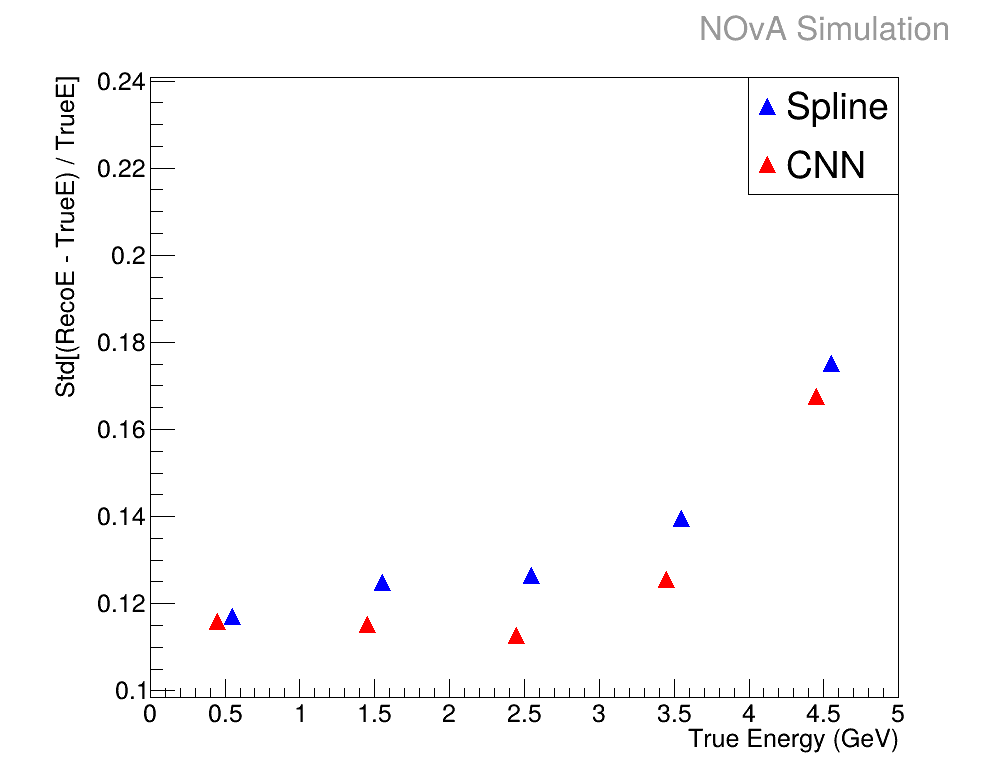
\includegraphics[width=0.7\textwidth]{images-lzhao/Numu_Energy_Resolution_RMSs.png}%
    }{%
        \fbox{\parbox[c][0.25\textheight][c]{0.7\textwidth}{\centering Neutrino Energy Resolution RMSs}}%
    }
    \caption{FHC ND Neutrino Energy Resolution.}
    \label{fig:lzhao-numu-energy-resolution}
\end{figure}

\section{A Complete List of Relevant Docdbs with Citations Including URL}

\bibliographystyle{unsrtnat}
\bibliography{summary-lzhao}

\end{document}

